%-------------------------------------------------------------------------------
% Applications of a Hybrid BEM-PINN Method to Inverse Wave Propagation Problems
% in Irregular Topographies
%-------------------------------------------------------------------------------
% Author: oscar-rincon
% Email: orincon@eafit.edu.co
% Creation date: 2024-03-15
% Version: 2.0 (first complete draft with numerical results)
%-------------------------------------------------------------------------------
\documentclass[11pt,twoside]{article}
%-------------------------------------------------------------------------------
% Import the style file
%-------------------------------------------------------------------------------
\usepackage{preprint}
\usepackage{booktabs}
% Macro to highlight text that still needs your input
\newcommand{\todo}[1]{\textcolor{red}{[#1]}}
%-------------------------------------------------------------------------------
% Document starts here
%-------------------------------------------------------------------------------
\begin{document}
\fancyhead[LE]{\thepage\, / \textit{Hybrid BEM–PINN Inversion in Irregular Topographies}}

% Set the page style to empty (no headers or footers)
\thispagestyle{empty}

%-------------------------------------------------------------------------------
% Title, Author, and Affiliation
%-------------------------------------------------------------------------------
\vspace{-2mm}
\begin{minipage}{15.0cm}
    \begin{center}
        \textbf{\large Applications of a Hybrid BEM–PINN Method to Inverse Wave Propagation Problems in Irregular Topographies}
    \end{center}
\end{minipage}
\begin{minipage}{0.0cm}
    \begin{center}
        %\hspace{-0.2cm}\includegraphics[width=2.8cm]{figs/format/eafit.pdf}
    \end{center}
\end{minipage}
\vspace{-2mm}
\vspace{0.6cm}

{\footnotesize\noindent O. Rincón-Cardeño$^1$, S. Montoya-Noguera$^2$, and N. Guarín-Zapata$^{1,*}$ \\
$^1$ Mathematical Applications in Science and Engineering Research Group, School of Applied Sciences and Engineering, Universidad EAFIT,
  Medellín, Colombia \\
$^2$ Nature and Cities Research Group, School of Applied Sciences and Engineering, Universidad EAFIT, Medellín, Colombia\\
  $^*$ Correspondence: nguarinz@eafit.edu.co}

%-------------------------------------------------------------------------------
% Abstract
%-------------------------------------------------------------------------------
\begin{tcolorbox}[colback=gray!20, colframe=gray!20, sharp corners]
    \begin{abstract}
        \vspace{-1mm}
        \noindent
Inferring subsurface geometry and material properties from seismic records of irregular topographies leads to ill-posed inverse problems. The boundary element method (BEM) handles wave radiation in semi-infinite domains exactly, while physics-informed neural networks (PINNs) offer flexible inversion through automatic differentiation. We investigate a hybrid BEM–PINN approach for inverse SH-wave problems, in which a Fourier-feature network represents the source densities of an indirect BEM and the geometric and material unknowns are trained jointly with the network. Three scenarios are considered: identification of an interface, reconstruction of the free surface, and joint estimation of geometry and material properties. We first reproduce the forward benchmarks of the underlying formulation (errors between $3.6\times10^{-4}$ and $4.7\times10^{-3}$), although its reported interpolation between frequencies was not reproduced. Our hypothesis was that, by never solving the BEM linear system, the hybrid method would reduce the cost of inversion. Compared with Levenberg–Marquardt and adjoint L-BFGS inversions that use the same discretization and data, it reaches the same accuracy but is two to three orders of magnitude slower. One training step costs about as much as one adjoint gradient, because both are dominated by kernel assembly, while the network needs thousands of steps instead of tens. The conclusion holds with preconditioned iterative solvers and in a three-dimensional extension, where the hybrid method needs 6 to 25 times more operator products. A basin-of-attraction test shows that the relaxed boundary conditions do not make it more robust than an adjoint solver with frequency continuation. The hypothesis is therefore rejected. The hybrid method is nevertheless a convenient prototyping tool: it requires only the action of the boundary operator and its automatic derivative, so new data types, parametrizations or operator back-ends can be tested without deriving adjoints, as we illustrate with amplitude-only data.
        \end{abstract}
\end{tcolorbox}

\noindent\textbf{Keywords:} Boundary element method; physics-informed neural networks; inverse problems; topographic effects; wave scattering

%-------------------------------------------------------------------------------
% Introduction
%-------------------------------------------------------------------------------
\section*{Introduction}\label{sec:introduction}
\fancyhead[RO]{\textit{Introduction}\, / \thepage}

\lettrine[lines=2,loversize=0.15,findent=0.4em,nindent=0em]{\textcolor{gray}{T}}{}opographic irregularities such as hills, ridges and canyons modify seismic ground motion, producing amplification and deamplification patterns that depend on surface geometry, subsurface structure and wave incidence angle \citep{Bard1982,Kawase1988}. Predicting these effects requires knowledge of the geometry and material properties of the medium, which are often uncertain or unavailable at field scale. Consequently, these parameters must be inferred from seismic records, leading to inverse problems involving geometric and material identification.

The boundary element method (BEM) is well suited to wave propagation in semi-infinite domains because it discretizes only boundaries and interfaces and naturally satisfies the radiation condition through appropriate Green's functions. Previous studies have used BEM to identify buried interfaces from surface-wave records \citep{Bignardi2012}, reconstruct free-surface geometries from scattering data \citep{Wang2018}, and jointly estimate the shape and material properties of elastic inclusions \citep{Bonnet2009}. However, BEM-based inversion relies on repeated forward solutions, making the optimization computationally demanding and potentially sensitive to noise and initial estimates \citep{Kallivokas2009,Chien2005}. Physics-informed neural networks (PINNs) offer an alternative for inverse parameter estimation by treating unknown quantities as trainable variables and computing derivatives through automatic differentiation \citep{Raissi2019}. They have been applied to wave propagation in anisotropic media and irregular topographies \citep{Song2022}, as well as full waveform inversion \citep{RashtBehesht2022}. However, accurately representing wave radiation in unbounded domains remains challenging. These complementary capabilities motivate the combination of physics-based numerical methods with machine learning to address problems that are challenging for either approach alone. In this context, hybrid BEM–PINN approaches have been explored in electromagnetics \citep{Barmada2024} and SH-wave scattering by complex topographies \citep{wu_novel_2026}. Although these studies demonstrate the potential of such combinations for forward wave propagation, their application to geometric and material inversion in seismic topographies remains unexplored.

In this work, we investigate the application of a hybrid BEM–PINN approach to three inverse seismic problems: (i) identification of the buried interface between a hill or sedimentary deposit and the underlying half-space, assuming known material properties; (ii) reconstruction of the free-surface geometry from scattering data; and (iii) joint identification of geometry and material properties. The motivation is to combine the capabilities of BEM for representing wave propagation in semi-infinite domains with the trainable parameter estimation capabilities of PINNs. Through these applications, we evaluate the suitability of this combination for inverse seismic characterization, considering reconstruction accuracy, sensitivity to measurement noise and computational cost. We test two hypotheses about where an advantage could come from. The first, which motivated this work, is computational: the hybrid method never solves the BEM system, so it could be cheaper than inversion schemes that require a converged forward solution at every iteration. The second concerns robustness: the hybrid method enforces the boundary conditions only through a penalty, so the forward and inverse problems are solved together in an enlarged search space, an idea that in full waveform inversion has been used to mitigate local minima \citep{Haber2000,vanLeeuwen2013}. We also examine a third, practical use: the hybrid method as a tool to prototype new inverse formulations without deriving adjoints.

A fair assessment requires a reference. We therefore (a) reproduce the forward benchmarks of the Fourier-feature BEM–PINN of \citet{wu_novel_2026}, on which our formulation builds, and (b) compare the hybrid inversion with two classical BEM inversion strategies modelled on the published works that motivate this study: the Gauss–Newton/Levenberg–Marquardt scheme with finite-difference sensitivities of \citet{Bignardi2012}, and the quasi-Newton scheme with adjoint shape and material gradients of \citet{Bonnet2009}. Those works address in-plane (P-SV) or three-dimensional elastodynamics and cannot be reproduced exactly with an antiplane model; we implement their algorithms for the SH problem considered here, with the same discretization, data and objective as the hybrid method, so that the comparison isolates the effect of the solution strategy.

%-------------------------------------------------------------------------------
\section{Geometric and Material Inversion in Irregular Topographies}\label{sec:problem_statement}
\fancyhead[RO]{\textit{Problem statement}\, / \thepage}
%-------------------------------------------------------------------------------

We consider the inverse characterization of an irregularity overlying or embedded in a semi-infinite elastic half-space. Seismic responses are assumed to be available at a set of observation points under prescribed wave excitation conditions. The objective is to estimate unknown geometric and material parameters by comparing observed responses with those predicted by the forward wave propagation model. Three inverse problem configurations are considered, as illustrated in Fig.~\ref{fig:problem_statement}.

\begin{figure*}[ht!]
    \centering
    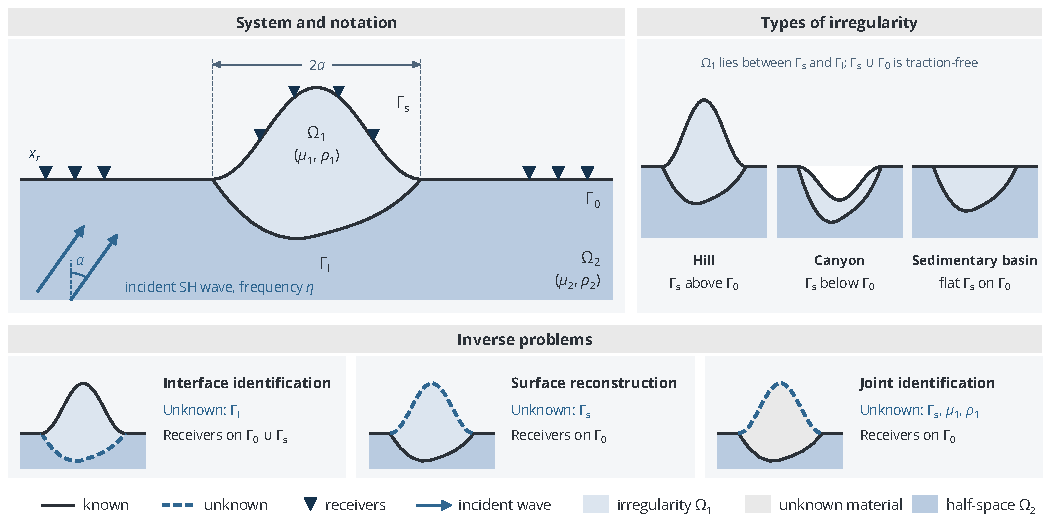
\includegraphics[width=6.5in]{figures/problem_statement.pdf}
\caption{Problem setting. Top left: an irregularity $\Omega_1$ with properties
  $(\mu_1,\rho_1)$, bounded by the free surface $\Gamma_s$ and the interface
  $\Gamma_I$, embedded in a half-space $\Omega_2$ with properties $(\mu_2,\rho_2)$
  and flat free surface $\Gamma_0$, excited by a plane SH wave with frequency
  $\eta$ and incidence angle $\alpha$; receivers $\mathbf{x}_r$ are placed on
  $\Gamma_0$ and, when it is known, on $\Gamma_s$. Top right: types of
  irregularity considered. Bottom: inverse problems; dashed orange lines and
  orange shading denote unknowns, and all other quantities are known.}
    \label{fig:problem_statement}
\end{figure*}

\noindent\textbf{Interface identification.} The free-surface geometry and the material properties of the irregularity and the half-space are known, while the geometry of the interface $\Gamma_I$ separating the two media is unknown. Because $\Gamma_s$ is known, receivers can be placed on it as well as on $\Gamma_0$.\\

\noindent\textbf{Surface reconstruction.} The interface and material properties are known, while the free-surface profile $\Gamma_s$ is unknown. Receivers can only be placed on the flat surface $\Gamma_0$, whose location is known.\\

\noindent\textbf{Joint identification.} Both the free-surface geometry and the material properties $(\mu_1,\rho_1)$ of the irregularity are unknown and must be estimated simultaneously. Geometric and material variations can produce similar effects on the wavefield, which increases the non-uniqueness of the problem.

%-------------------------------------------------------------------------------
\section{Hybrid BEM--PINN Inversion}\label{sec:methodology}
\fancyhead[RO]{\textit{Hybrid BEM–PINN inversion}\, / \thepage}
%-------------------------------------------------------------------------------

The inversion strategy extends the BEM--PINN formulation of \citet{wu_novel_2026} from forward scattering to geometric and material identification. A neural network represents the source densities of an indirect boundary element formulation, so the governing equation and the radiation condition are satisfied exactly by construction, while the boundary conditions and the seismic records enter as penalties in a single loss function. The geometric and material unknowns are treated as additional trainable variables and are updated jointly with the network weights (Fig.~\ref{fig:methodology_scheme}a). For comparison, Fig.~\ref{fig:methodology_scheme}b summarizes the adjoint-based reduced formulation described in Section~\ref{sec:baselines}.

\begin{figure*}[ht!]
    \centering
    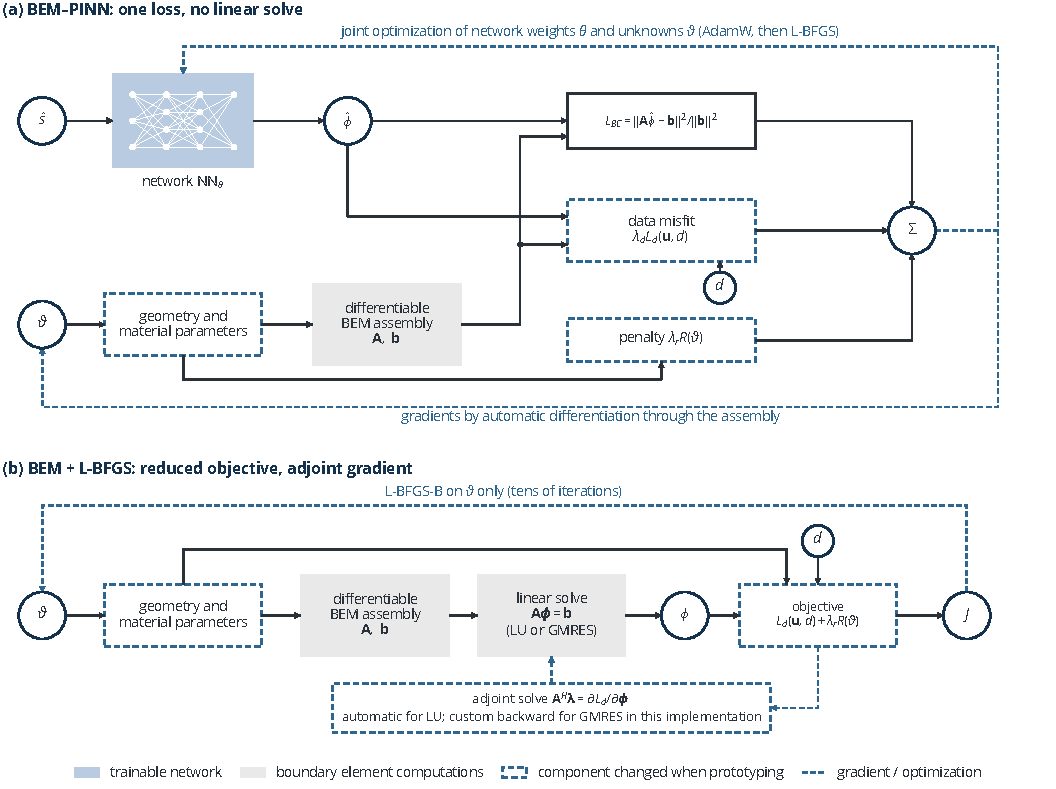
\includegraphics[width=6.5in]{figures/prototyping_workflow.pdf}
    \caption{Inversion workflows implemented on the same differentiable BEM.
      (a)~BEM--PINN: the network predicts source densities, and its weights
      $\theta$ and the geometric and material unknowns $\vartheta$ are updated
      jointly from a weighted loss combining boundary residuals, data misfit
      and regularization; no linear system is solved. (b)~BEM + L-BFGS with
      adjoint gradients: the BEM system is solved for each objective evaluation
      and differentiated to update $\vartheta$. Here $d$ denotes observed
      records and $\mathbf{u}$ the predicted receiver responses. Dashed boxes
      mark modular components that may change when prototyping a variant;
      dashed blue arrows indicate gradient or optimization paths.}
    \label{fig:methodology_scheme}
\end{figure*}

\subsection{Forward model}

We consider antiplane (SH) motion with time dependence $e^{i\omega t}$, horizontal coordinate $x$ and vertical coordinate $y$ pointing upwards, so that the half-space occupies $y<0$. The irregularity $\Omega_1$, with shear modulus $\mu_1$ and density $\rho_1$, is bounded by the free surface $\Gamma_s$ and the interface $\Gamma_I$. It may be a hill ($\Gamma_s$ above $\Gamma_0$), a canyon ($\Gamma_s$ below it) or a sedimentary basin (flat $\Gamma_s$). It is embedded in the half-space $\Omega_2$, with properties $(\mu_2,\rho_2)$, whose flat free surface outside the irregularity is $\Gamma_0$. The out-of-plane displacement $u_j$ in $\Omega_j$ satisfies
\begin{equation}
  \nabla^2 u_j + k_j^2 u_j = 0 \quad \text{in } \Omega_j,
  \qquad k_j = \frac{\omega}{\beta_j},\quad \beta_j = \sqrt{\mu_j/\rho_j},
  \qquad j = 1,2,
\end{equation}
subject to
\begin{equation}\label{eq:bcs}
  t_1 = 0 \ \text{on } \Gamma_s, \qquad
  t_2 = 0 \ \text{on } \Gamma_0, \qquad
  u_1 = u_2,\ \ t_1 = t_2 \ \text{on } \Gamma_I,
\end{equation}
where $t_j = \mu_j\,\partial u_j/\partial n$ is the traction, the normal $\mathbf{n}$ on $\Gamma_s$ points out of the solid, and $\mathbf{n}$ on $\Gamma_I$ points from $\Omega_1$ into $\Omega_2$. The excitation is a unit plane SH wave with incidence angle $\alpha$, measured from the vertical, and normalized frequency $\eta = \omega a/(\pi\beta_2)$, where $a$ is the half-width of the irregularity. In the absence of the irregularity, the incident and reflected waves form the free field
\begin{equation}
  u^{f\!f}(\mathbf{x}) = 2\, e^{-ik_2 x\sin\alpha}\cos(k_2 y\cos\alpha).
\end{equation}

Following the indirect BEM \citep{SanchezSesma1991,wu_novel_2026}, each field is written as a single-layer potential:
\begin{align}
  u_1(\mathbf{x}) &= \int_{\Gamma_s\cup\Gamma_I}
     \phi^{(1)}(\mathbf{x}_0)\, G_1(\mathbf{x},\mathbf{x}_0)\, dS(\mathbf{x}_0),
     & \mathbf{x}&\in\Omega_1, \label{eq:u1}\\
  u_2(\mathbf{x}) &= u^{f\!f}(\mathbf{x}) + \int_{\Gamma_I}
     \phi^{(2)}(\mathbf{x}_0)\, G_2(\mathbf{x},\mathbf{x}_0)\, dS(\mathbf{x}_0),
     & \mathbf{x}&\in\Omega_2. \label{eq:u2}
\end{align}
Here $G_1 = \frac{1}{4i\mu_1}H_0^{(2)}(k_1 r)$ is the full-space Green's function and
\begin{equation}
  G_2(\mathbf{x},\mathbf{x}_0) = \frac{1}{4i\mu_2}\Bigl[H_0^{(2)}(k_2 r) + H_0^{(2)}(k_2 \bar r)\Bigr]
\end{equation}
is the half-space Green's function, where $\bar r$ is the distance to the image of $\mathbf{x}_0$ with respect to $y=0$. With this choice $t_2=0$ on $\Gamma_0$ holds identically, so $\Gamma_0$ does not need to be discretized, unlike in \citet{wu_novel_2026}, where the flat surface is meshed up to eight wavelengths on each side of the topography. When the irregularity has no material of its own (an empty canyon), only $u_2$ is used and its density lives on $\Gamma_s$. Both representations satisfy the Helmholtz equation and the scattered part of $u_2$ satisfies the radiation condition, so only the conditions on $\Gamma_s$ and $\Gamma_I$ remain to be imposed.

The curves are divided into $N$ straight elements $\Delta S_l$ whose end points are clustered towards the corners where $\Gamma_s$, $\Gamma_I$ and $\Gamma_0$ meet, with a cosine law in the curve parameter. The element midpoints $\mathbf{x}_{0,l}$ serve as both source and collocation points. With a constant density per element,
\begin{equation}\label{eq:discrete}
  \begin{gathered}
  u_1(\mathbf{x}) = \sum_{l} \hat\phi^{(1)}_l\, G_{1,l}(\mathbf{x}),\qquad
  u_2(\mathbf{x}) = u^{f\!f}(\mathbf{x}) + \sum_{l} \hat\phi^{(2)}_l\, G_{2,l}(\mathbf{x}),\\
  G_{j,l}(\mathbf{x}) = \int_{\Delta S_l} G_j(\mathbf{x},\mathbf{x}_0)\, dS(\mathbf{x}_0),
  \end{gathered}
\end{equation}
and the tractions follow by differentiating $G_{j,l}$ along $\mathbf{n}$. Regular integrals use four-point Gauss quadrature. On the self-element, the logarithmic singularity of $G_j$ is removed by the substitution $t=\Delta S_l\,u^2/2$ before Gauss integration, and the traction receives the free term plus the principal value over the curved element,
\begin{equation}\label{eq:selfterm}
  T_{ll} = \pm\tfrac12 + \frac{\kappa_l\,\Delta S_l}{4\pi},
\end{equation}
where the sign is $+$ when $\mathbf{n}$ points out of the region whose field is evaluated and $\kappa_l$ is the signed curvature estimated from the neighbouring elements (it is set to zero at geometric corners). Without the curvature term, the principal value over each straight element vanishes and the error decays only linearly with the element size even for smooth boundaries.

Collecting the conditions~\eqref{eq:bcs} at the collocation points gives, for each excitation, a square linear system
\begin{equation}\label{eq:linear}
  \mathbf{A}(\vartheta,\eta)\,\boldsymbol{\phi} = \mathbf{b}(\vartheta,\eta,\alpha),
\end{equation}
whose rows are $t_1=0$ on $\Gamma_s$, $u_1-u_2=0$ and $t_1-t_2=0$ on $\Gamma_I$, with traction rows scaled by $1/(\mu_2 k_2)$. The conventional IBEM solves~\eqref{eq:linear} by LU factorization; the BEM--PINN never solves it.

\subsection{Network representation of the source densities}

The densities are represented by a fully connected network $\mathcal{N}_\theta$ with Fourier-feature input \citep{Tancik2020,wu_novel_2026}. Its input is the uniform boundary coordinate $\hat s = \arccos(1-2s)/\pi$, where $s\in[0,1]$ is the curve parameter shared by $\Gamma_s$ and $\Gamma_I$; with the cosine-clustered mesh, $\hat s$ is uniform in the element index, which removes the steep variation of the densities near the corners from the input space. For each of the $F\times J$ excitations $(\eta_f,\alpha_j)$ used in the inversion, the network has an output head with the real and imaginary parts of the three densities:
\begin{equation}
  \bigl(\hat\phi_s,\ \hat\phi_I^{(1)},\ \hat\phi_I^{(2)}\bigr)_{fj}(\hat s)
  = c_\phi\,\mathcal{N}_\theta\bigl(\gamma(\hat s)\bigr)_{fj},
  \qquad
  \gamma(\hat s) = \bigl[\sin(2\pi\mathbf{B}\hat s),\ \cos(2\pi\mathbf{B}\hat s)\bigr],
\end{equation}
where $\hat\phi_s$ and $\hat\phi_I^{(1)}$ are the restrictions of $\hat\phi^{(1)}$ to $\Gamma_s$ and $\Gamma_I$, and $\hat\phi_I^{(2)}$ is the density radiating into $\Omega_2$. The entries of $\mathbf{B}\in\mathbb{R}^{m}$ are drawn from $\mathcal{N}(0,\sigma^2)$ and kept fixed. The hidden layers are $\mathbf{h}^l = \mathrm{GELU}(\mathbf{W}^l\mathbf{h}^{l-1} + \mathbf{b}^l)$, with trainable parameters $\theta = \{\mathbf{W}^l,\mathbf{b}^l\}$. The constant $c_\phi$ is the root-mean-square of the Jacobi estimate $b_i/A_{ii}$ of the densities, which requires no linear solve. We also tested the formulation of \citet{wu_novel_2026}, in which the excitation parameters are additional network inputs; in the inversion setting it reached boundary residuals about one order of magnitude larger for the same training time, so we use one output head per excitation. The parametric input is retained in the forward frequency-interpolation test of Section~\ref{sec:forward}.

\subsection{Parametrization of the unknowns}

Both curves share the end points $x=\pm a$ and are written as
\begin{equation}\label{eq:shape}
  \Gamma_s:\ \bigl(x,\ y\bigr) = \Bigl(a(2s-1),\ \sum_{k=1}^{K}\xi_{s,k}\sin(k\pi s)\Bigr),
  \qquad
  \Gamma_I:\ \bigl(x,\ y\bigr) = \Bigl(a(2s-1),\ -\sum_{k=1}^{K}\xi_{I,k}\sin(k\pi s)\Bigr),
\end{equation}
so a truncated sine series with coefficients $\boldsymbol{\xi}_s,\boldsymbol{\xi}_I\in\mathbb{R}^K$ determines the geometry. The same parametrization covers the three types of irregularity: $\boldsymbol{\xi}_s$ describes a hill when it raises $\Gamma_s$ above $\Gamma_0$, a canyon when it lowers it, and a sedimentary basin when $\boldsymbol{\xi}_s=\mathbf{0}$. The vector of unknowns is (i)~$\vartheta = \boldsymbol{\xi}_I$, (ii)~$\vartheta = \boldsymbol{\xi}_s$, and (iii)~$\vartheta = (\boldsymbol{\xi}_s,\log\mu_1,\log\rho_1)$; all other quantities are fixed at their known values. Box constraints keep the first sine coefficient in $[0.05a, 1.5a]$, the higher ones in $[-0.3a, 0.3a]$, $\mu_1/\mu_2\in[0.1,3]$ and $\rho_1/\rho_2\in[0.3,3]$; they are enforced by projection after every update. The source points $\mathbf{x}_{0,l}(\vartheta)$, collocation points $\mathbf{x}_n(\vartheta)$, normals, element lengths, curvatures and the wavenumber $k_1(\mu_1,\rho_1)$ all depend differentiably on $\vartheta$; we implemented the Hankel functions $H_0^{(2)}$ and $H_1^{(2)}$ with analytical derivatives so that the whole assembly is differentiable in PyTorch \citep{Paszke2019}.

\subsection{Loss function and joint optimization}

For all excitations, the boundary conditions on $\Gamma_s$ and $\Gamma_I$ are imposed at the collocation points through the relative residual
\begin{equation}
  L_{BC} = \frac{\sum_{f,j}\bigl\|\mathbf{A}(\vartheta,\eta_f)\,\boldsymbol{\phi}_{fj}(\theta) - \mathbf{b}(\vartheta,\eta_f,\alpha_j)\bigr\|^2}
  {\sum_{f,j}\bigl\|\mathbf{b}(\vartheta,\eta_f,\alpha_j)\bigr\|^2},
\end{equation}
which contains the three residuals $t_1$ on $\Gamma_s$ and $u_1-u_2$, $t_1-t_2$ on $\Gamma_I$. The seismic records $u^{obs}_r = u^{obs}(\mathbf{x}_r;\eta_f,\alpha_j)$ enter through the data misfit. The receivers $\mathbf{x}_r$ lie on $\Gamma_0$ and, when the free surface is known (interface identification), also on $\Gamma_s$; the predicted response is $u = u_2$ on $\Gamma_0$ and $u = u_1$ on $\Gamma_s$:
\begin{equation}
  L_d = \frac{\sum_{r,f,j} |u(\mathbf{x}_r) - u^{obs}_r|^2}{\sum_{r,f,j} |u^{obs}_r|^2},
  \qquad
  R(\vartheta) = \sum_{k=1}^{K} k^{2p}\bigl(\xi_{s,k}^2 + \xi_{I,k}^2\bigr),
\end{equation}
where $R$ is a Sobolev-type penalty on the unknown coefficients that favours smooth geometries. The total loss is
\begin{equation}\label{eq:loss}
  L(\theta,\vartheta) = L_{BC} + \lambda_d L_d + \lambda_r R(\vartheta),
\end{equation}
and the network weights and the unknowns are updated jointly. Automatic differentiation gives $\nabla_\vartheta L$ through $k_1$ and through the kernels $G_j(\mathbf{x}_n(\vartheta),\mathbf{x}_{0,l}(\vartheta))$, so no shape derivatives or adjoint problems need to be derived.

Training proceeds in three stages. (1)~With $\vartheta$ fixed at the initial guess $\vartheta^0$, the network is trained on $L_{BC}$ alone, which amounts to a forward BEM solution; the matrices are assembled once. We use 1000 AdamW steps \citep{Loshchilov2019} with learning rate $10^{-3}$ followed by 100 L-BFGS iterations \citep{Liu1989} (at most 20 evaluations each, strong Wolfe line search). (2)~$\vartheta$ is released and~\eqref{eq:loss} is minimized with 1000 AdamW steps (learning rates $10^{-3}$ for $\theta$ and $3\times10^{-3}$ for $\vartheta$), starting with the two lowest frequencies and adding the others progressively during the first half of the stage. (3)~100 joint L-BFGS iterations refine the result. In stages 2 and 3 the BEM matrices are re-assembled at every loss evaluation because the geometry changes.

\subsection{Extension to three dimensions}\label{sec:method3d}

In three dimensions the SH problem has no counterpart, because P, SV and SH motions are coupled. To study how the method behaves when the boundary element model is three-dimensional, we consider the scalar analogue of the formulation above: the Helmholtz equation $\mu(\nabla^2 u + k^2 u)=0$ in the solid $z<0$, with traction-free (Neumann) surfaces. This is the model of acoustic scattering by a rigid surface, not of three-dimensional elastodynamics, and we use it only as a computational analogue. The half-space Green's function is
\begin{equation}
  G(\mathbf{x},\mathbf{x}_0) = \frac{1}{4\pi\mu}\left[\frac{e^{-ikr}}{r} + \frac{e^{-ik\bar r}}{\bar r}\right],
\end{equation}
so that the flat surface $z=0$ is again traction-free by construction, and the free field is the sum of an incident plane wave with polar angle $\alpha$ and azimuth $\varphi$ and its reflection. We study the reconstruction of the free surface of a canyon of radius $a$, parametrized over the unit disk $(u,v)$ as
\begin{equation}\label{eq:canyon3d}
  \Gamma_s:\ \bigl(x,y,z\bigr) = \Bigl(au,\ av,\ -\sum_{k=1}^{6}\xi_k\,\psi_k(u,v)\Bigr),\qquad
  \psi_k = (1-u^2-v^2)\,\{1,\ u,\ v,\ u^2-v^2,\ 2uv,\ u^2+v^2\}_k ,
\end{equation}
so the depth vanishes on the rim. The disk is triangulated on rings graded towards the rim; the triangles are flat, carry a constant density and are collocated at their centroids. Regular integrals use a three-point rule and, for pairs closer than 2.5 element sizes (including the images), a 28-point rule on four sub-triangles. On the self-triangle, the integral of $1/r$ is evaluated analytically and the remainder $(e^{-ikr}-1)/r$ numerically, and the traction receives the jump term and the principal value over the curved element, $\pm\frac12 + (\kappa_1+\kappa_2)\sqrt{\Delta S_l/\pi}/8$, with the curvature estimated from the normals of the neighbouring triangles. In the BEM--PINN, the network input is the centroid parameter $(u,v)$ of each triangle and, as in two dimensions, there is one output head per excitation.

%-------------------------------------------------------------------------------
\section{Reference BEM Inversion Methods}\label{sec:baselines}
\fancyhead[RO]{\textit{Reference BEM inversion}\, / \thepage}
%-------------------------------------------------------------------------------

The classical approach minimizes the data misfit of the converged forward model,
\begin{equation}\label{eq:classical}
  J(\vartheta) = L_d\bigl(\boldsymbol{\phi}(\vartheta)\bigr) + \lambda_r R(\vartheta),
  \qquad \mathbf{A}(\vartheta,\eta_f)\,\boldsymbol{\phi}_{fj} = \mathbf{b}(\vartheta,\eta_f,\alpha_j),
\end{equation}
so every evaluation of $J$ requires one assembly and one LU factorization per frequency. We use two solvers representative of the published BEM inversion literature, with the same discretization, parametrization, bounds, data and regularization as the BEM--PINN:

\noindent\textbf{BEM + Levenberg--Marquardt with finite differences (LM-FD).} Following \citet{Bignardi2012}, who used a Gauss--Newton update with a relaxation term and second-order finite-difference sensitivities, the residual vector $\mathbf{r}(\vartheta)$ (real and imaginary parts of the normalized misfits and the square root of the penalty) is linearized with a central finite-difference Jacobian, which costs $2P$ forward solutions for $P$ unknowns, and updated with the Levenberg--Marquardt rule \citep{Marquardt1963} with adaptive damping. Iterations stop when the misfit stagnates (relative change below $10^{-12}$) or the step falls below $10^{-8}$.

\noindent\textbf{BEM + L-BFGS with adjoint gradients (L-BFGS-adj).} Following \citet{Bonnet2009}, who computed shape and material sensitivities by adjoint and direct differentiation of the boundary integral equations and minimized the misfit with a quasi-Newton method, we obtain $\nabla_\vartheta J$ by reverse-mode differentiation through the assembly and the LU solve. This is algebraically the discrete adjoint method: each gradient costs one forward and one adjoint solve with the same factorization. The optimizer is L-BFGS-B \citep{Liu1989} with the box constraints above. As a control experiment for the joint problem, we also run L-BFGS-adj with the frequency continuation used by the BEM--PINN (successive solves with the two, three and four lowest frequencies, each warm-started).

%-------------------------------------------------------------------------------
\section{Numerical Experiments}\label{sec:experiments}
\fancyhead[RO]{\textit{Numerical experiments}\, / \thepage}
%-------------------------------------------------------------------------------

All quantities are dimensionless with $a=\mu_2=\rho_2=\beta_2=1$. All computations use double precision on the CPU of a laptop (Intel Core i9-13900H, 20 threads) with PyTorch~2.13 and SciPy~1.16; each process uses three or four threads. The installed PyTorch build could not use the GPU of the machine, so no GPU results are reported. The code and the scripts that produce every figure and table are available in the repository of this work.

\subsection{Verification and reproduction of the forward BEM--PINN}\label{sec:forward}

We first reproduce the forward benchmarks of \citet{wu_novel_2026}: a semicircular canyon, a semicircular hill of the same material as the half-space, and a V-shaped canyon with half-width $b=a$ and depth $d=a$, at $\eta=2$ and $\alpha=0^\circ,30^\circ,60^\circ,90^\circ$ (their Figs.~4--6 and Table~2). The canyon is compared with the exact solution of \citet{Trifunac1973}, which we evaluate as the mirror-symmetric problem of a cylindrical cavity in a full space. For the hill, the reference is our IBEM with 1200 elements per curve; it agrees with an independent solution obtained with the meshed-surface formulation described below to within $1.5\times10^{-3}$--$4.6\times10^{-3}$. For the V-shaped canyon, the half-space formulation cannot be used at $\eta=2$: the canyon and its image enclose a square of side $\sqrt2\,a$ whose interior Dirichlet eigenvalues include $k=2\pi$ (and $k=\pi$, i.e.\ $\eta=1$), so the single-layer system is singular there (Section~\ref{sec:discussion}). For this geometry we therefore use the formulation of \citet{wu_novel_2026}: the full-space Green's function, the flat surface meshed over eight wavelengths on each side with 240 elements per side, and 100 elements on the canyon. The reference is the same formulation with 400 elements on the canyon and 960 per side over sixteen wavelengths. We also verified the two-region formulation against the exact solution for a semicircular alluvial valley \citep{Trifunac1971} with $\beta_1/\beta_2=1/2$ and $\rho_1/\rho_2=2/3$, obtaining a maximum error of $5.6\times10^{-4}$ on the free surface with 400 elements per curve at $\eta=1$.

We use 100 elements on the topography, as \citet{wu_novel_2026}, and the network and training settings of their Section~3: six hidden layers of 150 neurons, $m=64$ Fourier features with $\sigma=1$, $4\times10^4$ AdamW steps with learning rate $10^{-3}$ and 200 L-BFGS iterations. The loss is the boundary-condition residual, and one network is trained per case. Accuracy is measured with the error of \citet{wu_novel_2026},
\begin{equation}
  \varepsilon = \frac{1}{M}\sum_{i=1}^{M}\frac{\bigl|\,|U_i| - |U_i^{ref}|\,\bigr|}{|U_i^{ref}|},
\end{equation}
over $M$ points on $\Gamma_0$ ($|x|\le 3a$) and on the topography. In the half-space formulation the network input is the curve parameter $s$; in the meshed-surface formulation it is the source position $(x_0,y_0)$, as in \citet{wu_novel_2026}.

\begin{figure*}[ht!]
    \centering
    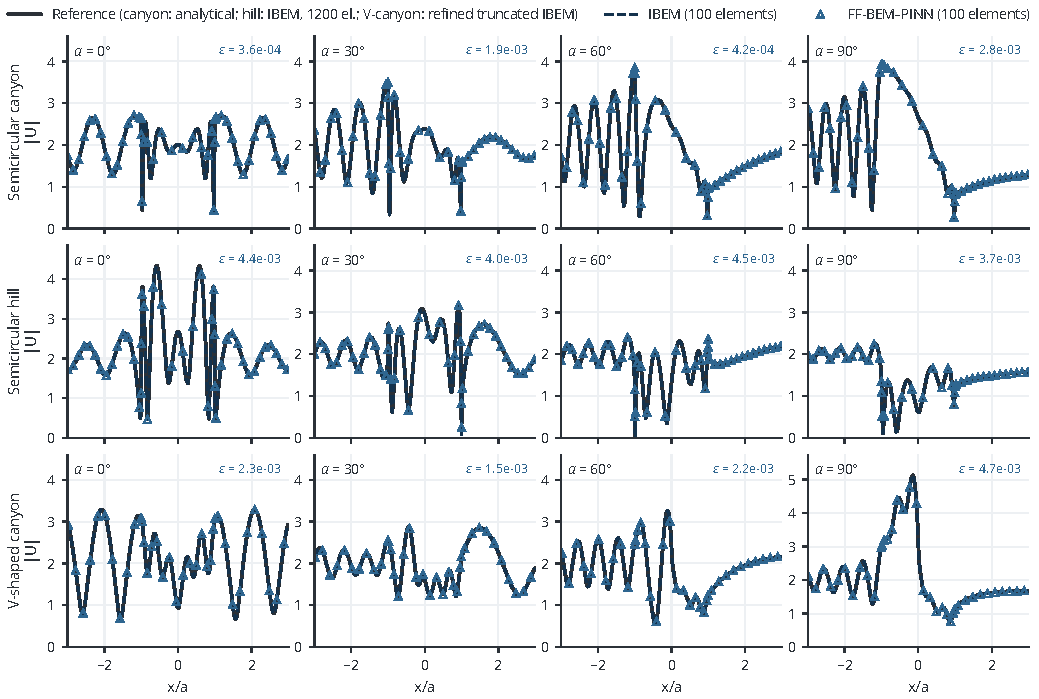
\includegraphics[width=6.5in]{figures/forward_reproduction.pdf}
    \caption{Reproduction of the forward benchmarks of \citet{wu_novel_2026} at $\eta=2$: surface displacement amplitude $|U|$ for the semicircular canyon (top), semicircular hill (middle) and V-shaped canyon (bottom). The error $\varepsilon$ of the FF-BEM--PINN against the reference is given in each panel.}
    \label{fig:forward}
\end{figure*}

\begin{table*}[ht!]
\centering
\caption{Forward benchmarks at $\eta=2$: error $\varepsilon$ and wall-clock time. Values for \citet{wu_novel_2026} are those reported in their Table~2 (FF PINN, GPU). Our IBEM time includes the assembly and the LU solve; our FF-BEM--PINN time includes the kernel assembly and training, with five runs sharing the CPU.}
\label{tab:forward}
\small
\begin{tabular}{llcccccc}
\toprule
 & & \multicolumn{2}{c}{Wu et al.\ (2026)} & \multicolumn{2}{c}{IBEM (this work)} & \multicolumn{2}{c}{FF-BEM--PINN (this work)}\\
\cmidrule(lr){3-4}\cmidrule(lr){5-6}\cmidrule(lr){7-8}
Topography & $\alpha$ & $\varepsilon$ & $R^2$ & $\varepsilon$ & time (s) & $\varepsilon$ & time (s)\\
\midrule
Semicircular canyon & 0$^\circ$ & $5.9\times10^{-3}$ & 0.997 & $3.6\times10^{-4}$ & 0.024 & $3.6\times10^{-4}$ & 454\\
 & 30$^\circ$ & $1.1\times10^{-2}$ & 0.993 & $1.9\times10^{-3}$ & 0.031 & $1.9\times10^{-3}$ & 365\\
 & 60$^\circ$ & $1.6\times10^{-2}$ & 0.994 & $4.2\times10^{-4}$ & 0.023 & $4.2\times10^{-4}$ & 455\\
 & 90$^\circ$ & $2.6\times10^{-2}$ & 0.994 & $2.8\times10^{-3}$ & 0.025 & $2.8\times10^{-3}$ & 423\\
\addlinespace
Semicircular hill & 0$^\circ$ & $1.8\times10^{-2}$ & 0.991 & $4.4\times10^{-3}$ & 0.068 & $4.4\times10^{-3}$ & 443\\
 & 30$^\circ$ & $1.6\times10^{-2}$ & 0.984 & $4.0\times10^{-3}$ & 0.046 & $4.0\times10^{-3}$ & 680\\
 & 60$^\circ$ & $1.3\times10^{-2}$ & 0.992 & $4.4\times10^{-3}$ & 0.048 & $4.5\times10^{-3}$ & 711\\
 & 90$^\circ$ & $2.0\times10^{-2}$ & 0.993 & $3.7\times10^{-3}$ & 0.026 & $3.7\times10^{-3}$ & 740\\
\addlinespace
V-shaped canyon & 0$^\circ$ & $2.5\times10^{-3}$ & 0.999 & $2.3\times10^{-3}$ & 0.173 & $2.3\times10^{-3}$ & 890\\
 & 30$^\circ$ & $5.6\times10^{-3}$ & 0.999 & $1.5\times10^{-3}$ & 0.137 & $1.5\times10^{-3}$ & 885\\
 & 60$^\circ$ & $2.1\times10^{-2}$ & 0.994 & $2.2\times10^{-3}$ & 0.155 & $2.2\times10^{-3}$ & 877\\
 & 90$^\circ$ & $2.3\times10^{-2}$ & 0.997 & $4.7\times10^{-3}$ & 0.161 & $4.7\times10^{-3}$ & 890\\
\bottomrule
\end{tabular}

\end{table*}

Figure~\ref{fig:forward} and Table~\ref{tab:forward} summarize the results. The FF-BEM--PINN converges to the same solution as the direct IBEM solve: in all twelve cases the two errors differ by less than 2.2\% of their value, so the remaining error is the discretization error of the 100-element mesh and not a training error. Our errors range from $3.6\times10^{-4}$ to $4.7\times10^{-3}$, against $2.5\times10^{-3}$ to $2.6\times10^{-2}$ reported by \citet{wu_novel_2026}. For the canyon and the hill the improvement comes mainly from the half-space Green's function, which removes the truncated flat surface, the curvature correction~\eqref{eq:selfterm}, which restores the convergence order, and the graded mesh, which resolves the corner behaviour. For the V-shaped canyon we used their formulation, and the difference comes from the reference: we compare with a refined solution of the same formulation, whereas \citet{wu_novel_2026} compare with the analytical solution of \citet{TsaurChang2008}. The characteristic features of their figures are recovered, for instance the peak $|U|\approx5$ near $x\approx-0.1b$ for grazing incidence on the V-shaped canyon. The direct IBEM solution takes between 0.02 and 0.17~s, while training the network takes 6 to 15 minutes on the same hardware (with five trainings sharing the CPU).

\noindent\textbf{Frequency as network input.} \citet{wu_novel_2026} also trained one network with the frequency as an additional input over $\eta\in[4.0,4.5]$, at three training frequencies, and reported 7.2~h for the FF PINN against 9.9~h for their BEM to evaluate 11 frequencies (their Table~3). We repeated this test for the V-shaped canyon at $\alpha=0^\circ$ with their formulation (flat surface meshed over eight wavelengths of the lowest frequency, 240 elements per side, 100 elements on the canyon), the input $(x_0,y_0,\eta)$, eight hidden layers of 200 neurons, $m=128$, $\sigma=1$, $2\times10^4$ AdamW steps and 100 L-BFGS iterations. The network is trained at the two ends and the centre of the band and evaluated at 11 equally spaced frequencies. We used two bands: $\eta\in[1.0,1.5]$, and $\eta\in[1.0,1.125]$, whose relative width equals that of the band of \citet{wu_novel_2026}. Figure~\ref{fig:frequency} shows the results. At the three training frequencies the network reproduces the IBEM solution ($\varepsilon\le1.1\times10^{-3}$), but between them the error grows to 30\% in both bands (mean $1.8\times10^{-1}$ and $1.9\times10^{-1}$ over the eight non-training frequencies), and adding weight decay (coefficient 0.1), which improved the interpolation over the incidence angle in \citet{wu_novel_2026}, does not change this ($2.0\times10^{-1}$). We therefore could not reproduce the interpolation accuracy reported by \citet{wu_novel_2026} (average $\varepsilon=1.26\%$); the boundary-condition loss constrains the densities only at the training frequencies, and with the settings we tested nothing in the training makes the network interpolate correctly between them. Some settings of the original study for this test (the Fourier scale and the normalization of the inputs) are not stated, which may explain part of the difference. Regarding cost, the IBEM evaluates the 11 frequencies in 0.7--1.8~s, whereas the training takes 18--22 minutes, so the time advantage reported by \citet{wu_novel_2026} (7.2~h against 9.9~h) is not observed with our implementation.

\begin{figure*}[ht!]
    \centering
    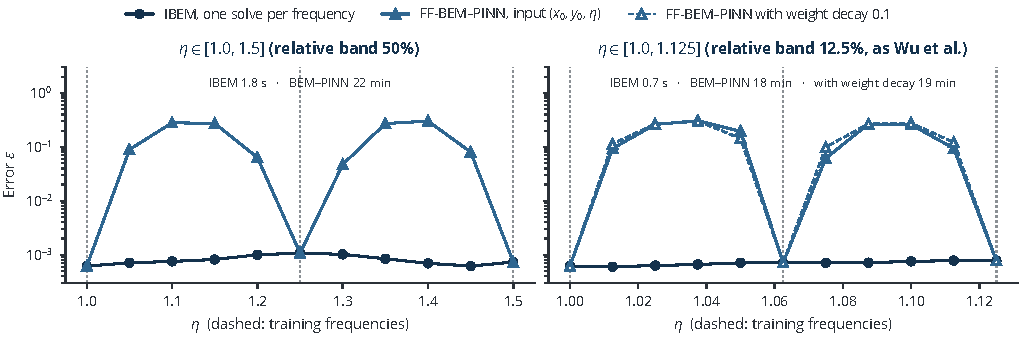
\includegraphics[width=6.5in]{figures/frequency_input.pdf}
    \caption{Frequency as network input (V-shaped canyon, $\alpha=0^\circ$): error $\varepsilon$ of the FF-BEM--PINN trained at three frequencies (dashed lines) and of the IBEM, which solves every frequency directly. The legends give the total wall-clock time of each method for the 11 frequencies.}
    \label{fig:frequency}
\end{figure*}

\subsection{Inverse problems: set-up}\label{sec:setup}

The true irregularity is a hill with $\mu_1=0.5$ and $\rho_1=0.8$ ($\beta_1/\beta_2=0.79$), with free surface $\boldsymbol{\xi}_s = (0.70, 0.10, -0.06, 0.04)$ and interface $\boldsymbol{\xi}_I = (0.50, 0.15, 0.08, -0.03)$ in~\eqref{eq:shape} ($K=4$). The data are the complex displacements at $\eta\in\{0.25,0.5,0.75,1.0\}$ and $\alpha\in\{-30^\circ,0^\circ,30^\circ\}$ at 20 receivers on $\Gamma_0$, ten on each side at $1.15a\le|x|\le 3a$, plus nine receivers on $\Gamma_s$ for interface identification. To avoid an inverse crime, the data are computed with 120 elements per curve and eight Gauss points, three times finer than the 40 elements per curve used by all inversion methods. Noise is added as $u^{obs}_r = u_r(1+\sigma_n\epsilon_r)$, with $\epsilon_r$ a standard complex Gaussian variable and $\sigma_n\in\{0, 1\%, 3\%\}$; the same noisy data set is used by all solvers. All methods start from $\boldsymbol{\xi}_s^0=(0.35,0,0,0)$, $\boldsymbol{\xi}_I^0=(0.25,0,0,0)$ and, for joint identification, a homogeneous medium $\mu_1^0=\rho_1^0=1$; the regularization parameters are $\lambda_r=10^{-5}$, $p=1$ and $\lambda_d=1$. The accuracy of a reconstructed curve is the relative $L^2$ error $\|y-y^{true}\|/\|y^{true}\|$ of the unknown curve, and the material errors are relative errors. The BEM--PINN uses four hidden layers of 150 neurons, $m=64$ and $\sigma=3$.

\subsection{Inverse problems: accuracy and computational time}\label{sec:inverse_results}

\begin{table*}[ht!]
\centering
\caption{Inversion results. Error: relative $L^2$ error of the unknown curve (largest of shape and material errors for joint identification). Solves: number of forward evaluations of~\eqref{eq:classical} (assembly and LU solve for four frequencies); assemblies: number of loss evaluations with re-assembly of the BEM matrices. Classical solvers ran alone on the machine; three BEM--PINN runs shared it.}
\label{tab:inverse}
\scriptsize
\setlength{\tabcolsep}{4pt}
\begin{tabular}{llccccccccc}
\toprule
 & & \multicolumn{3}{c}{BEM + LM (FD Jacobian)} & \multicolumn{3}{c}{BEM + L-BFGS (adjoint)} & \multicolumn{3}{c}{BEM--PINN (this work)}\\
\cmidrule(lr){3-5}\cmidrule(lr){6-8}\cmidrule(lr){9-11}
Problem & noise & error & time (s) & solves & error & time (s) & solves & error & time (s) & assemblies\\
\midrule
Interface identification & 0\% & 1.59\% & 0.839 & 64 & 1.59\% & 0.543 & 14 & 0.99\% & 259 & 3217\\
 & 1\% & 1.65\% & 0.822 & 64 & 1.65\% & 0.587 & 14 & 1.26\% & 262 & 3219\\
 & 3\% & 1.79\% & 0.933 & 71 & 1.79\% & 0.609 & 14 & 1.91\% & 259 & 3210\\
\addlinespace
Surface reconstruction & 0\% & 0.35\% & 0.997 & 73 & 0.35\% & 0.382 & 14 & 0.35\% & 204 & 3229\\
 & 1\% & 0.38\% & 0.951 & 73 & 0.38\% & 0.371 & 14 & 0.43\% & 203 & 3245\\
 & 3\% & 0.47\% & 0.802 & 64 & 0.47\% & 0.341 & 14 & 0.61\% & 202 & 3227\\
\addlinespace
Joint identification & 0\% & 0.75\% & 1.83 & 144 & 29.72\% & 1.75 & 67 & 0.65\% & 199 & 3216\\
 & 1\% & 0.50\% & 1.92 & 144 & 41.19\% & 2.05 & 79 & 0.56\% & 197 & 3223\\
 & 3\% & 0.34\% & 2.13 & 144 & 0.34\% & 1.36 & 54 & 0.47\% & 198 & 3217\\
\bottomrule
\end{tabular}

\end{table*}

\begin{figure*}[ht!]
    \centering
    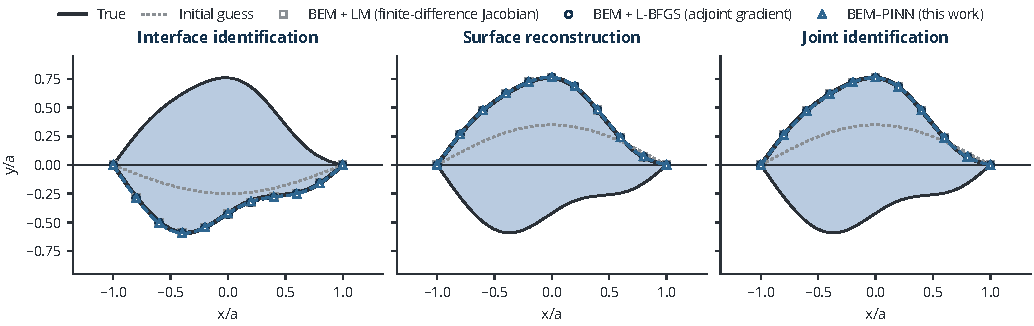
\includegraphics[width=6.5in]{figures/inverse_reconstruction.pdf}
    \caption{Reconstructed curves for 3\% noise. Interface identification shows $\Gamma_I$; surface reconstruction and joint identification show $\Gamma_s$. The shaded region is the true irregularity.}
    \label{fig:reconstruction}
\end{figure*}

Table~\ref{tab:inverse} and Figs.~\ref{fig:reconstruction}--\ref{fig:convergence} summarize the inversions. In terms of accuracy, the BEM--PINN performs as well as the classical solvers in the three problems. For interface identification its errors are 0.99\%, 1.26\% and 1.91\% for 0\%, 1\% and 3\% noise, against 1.59\%, 1.65\% and 1.79\% for both classical solvers; for surface reconstruction they are 0.35\%, 0.43\% and 0.61\%, against 0.35\%, 0.38\% and 0.47\%. The reconstructed curves are visually indistinguishable from the true ones for all solvers (Fig.~\ref{fig:reconstruction}). Without noise, the errors of the classical solvers are not zero because the data come from a three times finer mesh: with data computed on the inversion mesh (an inverse crime), L-BFGS recovers the interface with an error of 0.03\% and the free surface with 0.002\%, and removing the regularization does not change the errors with the fine-mesh data. The interface error floor is about four times larger than the surface one because the buried interface has a weaker effect on the surface response. The slightly lower error of the BEM--PINN without noise for interface identification is consistent with this interpretation: the network densities do not satisfy the 40-element system exactly (the final relative residual $L_{BC}$ is of order $10^{-5}$), which gives the data misfit some freedom to absorb discretization error; the advantage disappears as noise increases.

Joint identification is the most informative case (Table~\ref{tab:joint}). LM-FD recovers the free surface and the material properties at all noise levels, with shape errors of 0.22--0.23\% and material errors below 0.8\%. L-BFGS-adj, started from the same homogeneous initial guess, stops in a local minimum without noise and with 1\% noise (shape errors of 30\% and 41\%) and only reaches the solution with 3\% noise. The BEM--PINN reaches the solution at all noise levels (largest error 0.65\%). However, the BEM--PINN also uses frequency continuation. When L-BFGS-adj is run with the same continuation, solving successively with the two, three and four lowest frequencies and warm-starting each stage, it reaches the solution at all noise levels in 1.5~s (Table~\ref{tab:joint} and Fig.~\ref{fig:convergence}). The robustness of the BEM--PINN in this test is therefore explained by the continuation strategy and not by the network representation itself; Section~\ref{sec:basin} tests this conclusion over a range of initial guesses and frequency bands.

In terms of computational time, the classical solvers need between 0.3~s and 2.1~s per inversion, with 14 to 144 forward solutions, whereas the BEM--PINN needs 197--262~s, that is, 100 to 550 times more (Fig.~\ref{fig:accuracy_time}). About 35~s of the BEM--PINN time is the pre-training at the initial guess, that is, the network version of a single forward solution that the IBEM obtains in about 0.01~s (shaded interval in Fig.~\ref{fig:convergence}). The rest corresponds to 1000 AdamW steps and about 2200 L-BFGS evaluations, each of which re-assembles the BEM matrices.

\begin{figure*}[ht!]
    \centering
    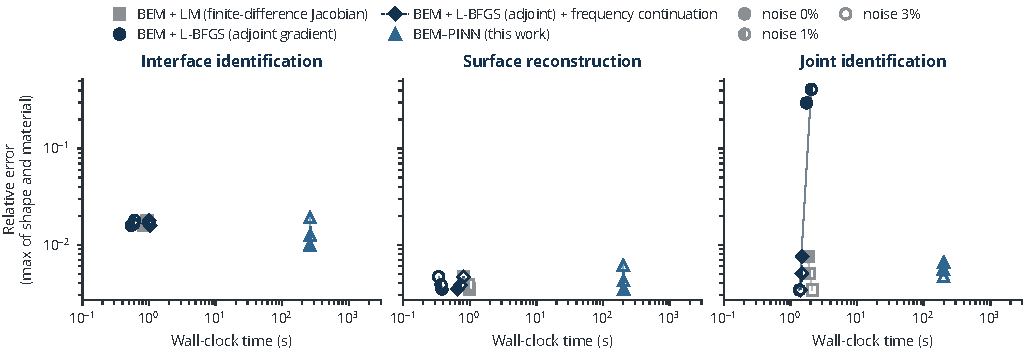
\includegraphics[width=6.5in]{figures/inverse_accuracy_time.pdf}
    \caption{Accuracy against wall-clock time for the three inverse problems and three noise levels. Each marker is one inversion; lines connect the noise levels of each solver.}
    \label{fig:accuracy_time}
\end{figure*}

\begin{figure*}[ht!]
    \centering
    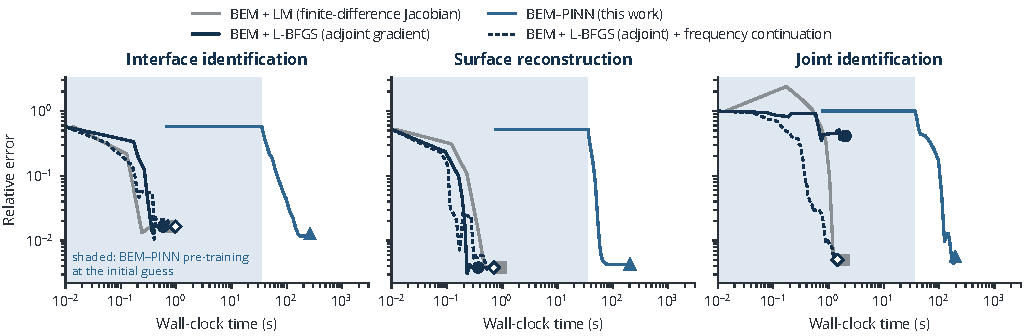
\includegraphics[width=6.5in]{figures/inverse_convergence.pdf}
    \caption{Convergence histories for 1\% noise: relative error of the unknowns against wall-clock time. The shaded interval is the BEM--PINN pre-training (forward solution at the initial guess).}
    \label{fig:convergence}
\end{figure*}

\begin{table}[ht!]
\centering
\caption{Joint identification: errors of the free surface and of the material properties.}
\label{tab:joint}
\scriptsize
\setlength{\tabcolsep}{4pt}
\begin{tabular}{llcccc}
\toprule
Solver & noise & shape & $\mu_1$ & $\rho_1$ & time (s)\\
\midrule
BEM + LM (finite-difference Jacobian) & 0\% & 0.23\% & 0.75\% & 0.37\% & 1.83\\
 & 1\% & 0.22\% & 0.50\% & 0.13\% & 1.92\\
 & 3\% & 0.22\% & 0.00\% & 0.34\% & 2.13\\
\addlinespace
BEM + L-BFGS (adjoint gradient) & 0\% & 29.72\% & 9.47\% & 1.60\% & 1.75\\
 & 1\% & 41.19\% & 38.92\% & 1.26\% & 2.05\\
 & 3\% & 0.22\% & 0.00\% & 0.34\% & 1.36\\
\addlinespace
BEM + L-BFGS (adjoint), frequency continuation & 0\% & 0.23\% & 0.75\% & 0.37\% & 1.5\\
 & 1\% & 0.22\% & 0.50\% & 0.13\% & 1.48\\
 & 3\% & 0.22\% & 0.00\% & 0.34\% & 1.41\\
\addlinespace
BEM--PINN (this work) & 0\% & 0.47\% & 0.65\% & 0.08\% & 199\\
 & 1\% & 0.27\% & 0.56\% & 0.12\% & 197\\
 & 3\% & 0.47\% & 0.22\% & 0.40\% & 198\\
\bottomrule
\end{tabular}

\end{table}

\subsection{Computational cost}\label{sec:cost}

\begin{figure*}[ht!]
    \centering
    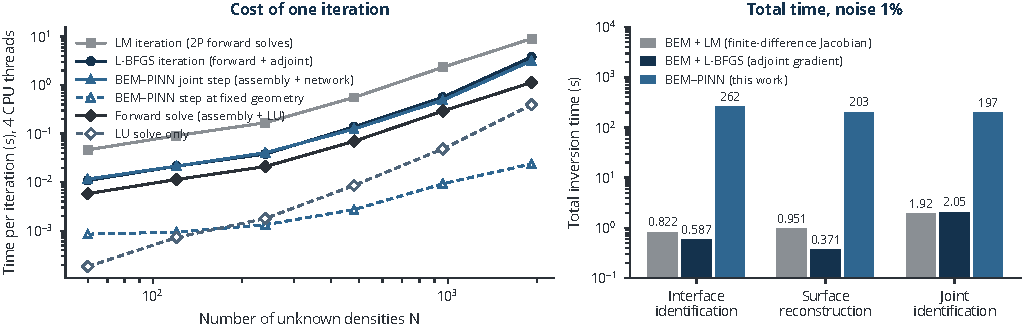
\includegraphics[width=6.5in]{figures/computational_cost.pdf}
    \caption{Left: time per iteration against the number of unknown densities $N$ (three density sets of $N/3$ elements, four frequencies, three incidence angles). Right: total inversion time for 1\% noise.}
    \label{fig:cost}
\end{figure*}

Figure~\ref{fig:cost} explains these differences. For the sizes considered, the cost of one forward evaluation is dominated by the assembly of the integrated kernels, which grows as $N^{1.8}$ in the measured range (asymptotically $N^2$), while the LU solve grows as $N^{2.8}$ (asymptotically $N^3$) but represents only 3\% of the forward cost for $N=60$ unknown densities and 35\% for $N=1920$; extrapolating the measured constants, the solve would dominate only above about 3600 unknowns. A joint BEM--PINN step has to re-assemble the kernels and differentiate through them, so it costs the same as one L-BFGS-adj iteration (forward plus adjoint) at every size, and an LM-FD iteration costs $2P$ forward solutions. Avoiding the linear solve brings no saving per iteration in this regime, and the BEM--PINN needs about 3200 assemblies, 20 to 230 times more than the forward evaluations of the classical solvers. A BEM--PINN step at fixed geometry, without re-assembly, is much cheaper (0.8--24~ms) and is the regime in which the network formulation is efficient; this situation occurs in forward parametric studies, not in shape inversion, where the geometry changes at every step.

\subsection{Iterative solvers: a regime favourable to the hybrid method?}\label{sec:iterative}

The comparison above uses LU factorizations, which are only possible while the dense matrix fits in memory and its factorization is affordable. For large models the classical solvers must instead solve every forward and adjoint problem iteratively, without storing the matrix, and the relevant cost becomes the number of products with $\mathbf{A}$ and $\mathbf{A}^H$; one such product is the operation that a fast multipole or hierarchical-matrix implementation accelerates. The hybrid method needs exactly two products per right-hand side and loss evaluation (one with $\mathbf{A}$ for the residual and one with $\mathbf{A}^H$ for its gradient) and never converges an individual forward problem, so this is the regime where it could pay off. We repeated surface reconstruction with 1\% noise for $N=120$ to 960 unknown densities, solving the forward and adjoint problems of the classical solvers with GMRES \citep{Saad1986} to a relative residual of $10^{-10}$, with a Jacobi preconditioner whose diagonal is given analytically by the self terms (unpreconditioned GMRES needed 2.2 times more iterations at $N=480$). Figure~\ref{fig:iterative} shows the results. The number of products of the BEM--PINN is independent of $N$ (about $1.5\times10^5$ for the whole inversion, half of them in the pre-training), whereas that of the classical solvers grows slowly, as $N^{0.24}$ for L-BFGS-adj (from $1.5\times10^4$ to $2.5\times10^4$) and from $2.8\times10^4$ to $4.0\times10^4$ for LM-FD. The hybrid method therefore needs 6 to 10 times more products than L-BFGS-adj in this range, and the fitted trends would only cross at about $1.6\times10^6$ unknowns. Moreover, with a fixed training budget the error of the BEM--PINN stagnates at 0.24\% when the mesh is refined, while that of the classical solvers keeps decreasing with the discretization error (0.064\% for $N=960$), so matching their accuracy on finer meshes would require more training steps.

\begin{figure*}[ht!]
    \centering
    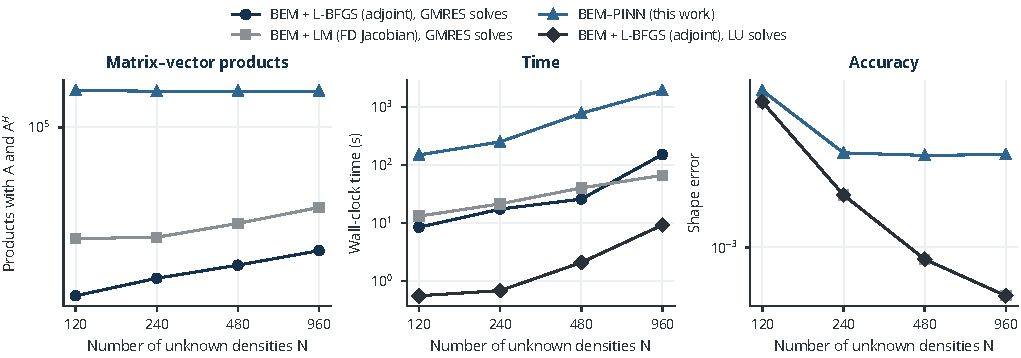
\includegraphics[width=6.5in]{figures/iterative_regime.pdf}
    \caption{Iterative regime (surface reconstruction, 1\% noise): total number of products with $\mathbf{A}$ and $\mathbf{A}^H$, wall-clock time and shape error against the number of unknown densities. The classical solvers use Jacobi-preconditioned GMRES for every forward and adjoint solve; the LU-based L-BFGS solver is shown for reference.}
    \label{fig:iterative}
\end{figure*}

\subsection{Three-dimensional canyon}\label{sec:three_d}

We verified the three-dimensional formulation against the exact solution for a rigid hemispherical canyon of radius $a$, obtained as a rigid sphere illuminated by the incident wave and its mirror image. At 72 points of $z=0$ with $1.25a\le r\le 2.5a$, the maximum relative error is $5.4\times10^{-3}$, $1.7\times10^{-3}$ and $8.4\times10^{-4}$ for meshes of 216, 600 and 1536 triangles at $\eta=0.5$ and vertical incidence, and $1.0\times10^{-2}$, $3.1\times10^{-3}$ and $9.4\times10^{-4}$ at $\eta=0.75$ and $\alpha=30^\circ$; the estimated curvature sum is within 10\% of the exact value $2/a$. Note that the hemisphere and its image form a sphere whose first interior Dirichlet eigenvalue is $k=\pi$ ($\eta=1$), which we avoid.

The inverse problem is the reconstruction of the canyon~\eqref{eq:canyon3d} with $\boldsymbol{\xi} = (0.55, 0.12, -0.08, 0.06, -0.04, 0.10)$ from the displacements at 36 receivers on $z=0$ (three rings of radius $1.25a$, $1.75a$ and $2.5a$ with 12 receivers each), for $\eta\in\{0.25, 0.5, 0.75\}$ and three plane waves ($\alpha=0^\circ$; $\alpha=30^\circ$ with $\varphi=0^\circ$ and $90^\circ$). The data are computed with 1536 triangles and the inversions use 384, starting from $\boldsymbol{\xi}^0=(0.30,0,0,0,0,0)$, with the penalty $R=\sum_k d_k^2\xi_k^2$, where $d_k$ is the polynomial degree of $\psi_k$ plus one, and the same settings as in two dimensions otherwise ($\sigma=1$ for the Fourier features). Table~\ref{tab:three_d} and Fig.~\ref{fig:three_d} summarize the results. The three classical solvers converge to the same reconstruction, with depth errors of 0.93\%, 1.99\% and 4.59\% for 0\%, 1\% and 3\% noise, in 6 to 15~s. The errors grow faster with noise than in two dimensions because only low frequencies are used and the canyon has a weak signature in the data: the misfit of the initial guess is only $2.7\times10^{-3}$. L-BFGS-adj needs 23 objective evaluations, that is, about 4600 products with $\mathbf{A}$ and $\mathbf{A}^H$ when GMRES is used. The BEM--PINN reaches errors of 5.5\%, 6.0\% and 7.2\% after 29 minutes and about 6500 loss evaluations ($1.15\times10^5$ products, 25 times more than L-BFGS-adj with GMRES), so in three dimensions it is less accurate than the classical solvers even without noise. The training history explains why. The pre-training at the initial guess reaches a relative residual $L_{BC}$ of only $1.5\times10^{-4}$, against $7\times10^{-6}$ in two dimensions, and during the joint training the residual ($5.6\times10^{-5}$ at the end) remains larger than the data misfit ($8.5\times10^{-6}$), which falls below the misfit of the true geometry on the inversion mesh ($9.3\times10^{-5}$). The network therefore fits the data partly through densities that do not satisfy the boundary conditions instead of through the geometry, and the error was still decreasing when the training stopped. A larger weight on $L_{BC}$ or a longer training would reduce this bias, at a further increase in cost.

\begin{table}[ht!]
\centering
\caption{Three-dimensional canyon reconstruction: relative $L^2$ error of the depth, wall-clock time, number of forward evaluations (classical) or loss evaluations (BEM--PINN), and number of products with $\mathbf{A}$ and $\mathbf{A}^H$ (iterative solvers and BEM--PINN).}
\label{tab:three_d}
\scriptsize
\setlength{\tabcolsep}{4pt}
\begin{tabular}{llcccc}
\toprule
Solver & noise & error & time (s) & evaluations & products\\
\midrule
BEM + LM (FD Jacobian), LU & 0\% & 0.93\% & 10.6 & 79 & --\\
 & 1\% & 1.99\% & 12.8 & 92 & --\\
 & 3\% & 4.59\% & 15.2 & 105 & --\\
\addlinespace
BEM + L-BFGS (adjoint), LU & 0\% & 0.93\% & 8.66 & 23 & --\\
 & 1\% & 1.99\% & 5.63 & 23 & --\\
 & 3\% & 4.59\% & 7.27 & 23 & --\\
\addlinespace
BEM + L-BFGS (adjoint), GMRES & 0\% & 0.93\% & 13.5 & 23 & 4603\\
 & 1\% & 1.99\% & 11.3 & 23 & 4619\\
 & 3\% & 4.59\% & 14.8 & 23 & 4602\\
\addlinespace
BEM--PINN (this work) & 0\% & 5.50\% & 1.74e+03 & 6475 & 115050\\
 & 1\% & 6.00\% & 1.75e+03 & 6479 & 115122\\
 & 3\% & 7.17\% & 1.74e+03 & 6485 & 115230\\
\bottomrule
\end{tabular}

\end{table}

\begin{figure*}[ht!]
    \centering
    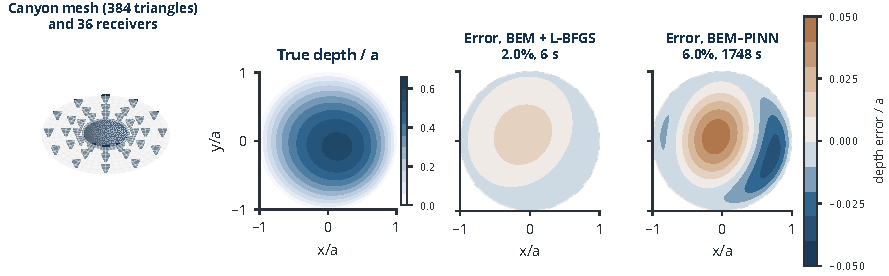
\includegraphics[width=6.5in]{figures/three_d_reconstruction.pdf}
    \caption{Three-dimensional canyon reconstruction with 1\% noise. Left: true canyon (inversion mesh) and receivers. Right: true depth and depth errors of the reconstructions over the canyon footprint, with the relative $L^2$ error and the wall-clock time.}
    \label{fig:three_d}
\end{figure*}

\begin{figure*}[ht!]
    \centering
    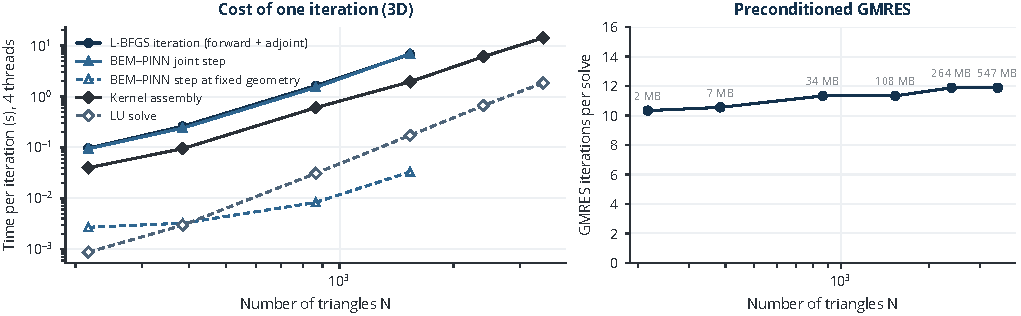
\includegraphics[width=6.5in]{figures/scaling_3d.pdf}
    \caption{Three-dimensional cost study (canyon, three frequencies, three excitations). Left: time per iteration against the number of triangles. Right: Jacobi-preconditioned GMRES iterations per solve, with the memory of the three dense matrices.}
    \label{fig:scaling3d}
\end{figure*}

The cost study of Fig.~\ref{fig:scaling3d} confirms the two-dimensional analysis. The assembly of the integrated kernels dominates the cost: for 3456 triangles it takes 14~s per objective evaluation against 1.8~s for the three LU solves, and, extrapolating the measured exponents, the dense solve would dominate only above roughly $2.7\times10^4$ triangles. A joint BEM--PINN step costs the same as an adjoint gradient at every size (6.9~s and 6.8~s for 1536 triangles). The three-dimensional systems are well conditioned: Jacobi-preconditioned GMRES converges in 10 to 12 iterations independently of the mesh, so even when the matrix (547~MB for three frequencies with 3456 triangles) can no longer be factorized or stored, an iterative classical solver needs a few hundred products per objective evaluation, far fewer than the thousands of loss evaluations of the hybrid method.

\subsection{Basin of attraction: is the hybrid method more robust?}\label{sec:basin}

The previous sections reject the hypothesis of a lower computational cost. A different advantage could come from the formulation itself. The classical solvers minimize the reduced objective~\eqref{eq:classical}, in which the densities are the exact solution of the BEM system for the current geometry, whereas the BEM--PINN minimizes~\eqref{eq:loss}, in which the boundary conditions are only penalized. The latter is an all-at-once formulation \citep{Haber2000} in an enlarged search space, similar to wavefield reconstruction inversion, which mitigates local minima in full waveform inversion because the forward equations do not have to be satisfied exactly away from the solution \citep{vanLeeuwen2013}. The inversions of Section~\ref{sec:inverse_results} cannot test this, because they start from a single initial guess and use low frequencies, for which the objective is nearly convex in the surface problem. We therefore repeated surface reconstruction with 1\% noise from eight initial guesses, $\boldsymbol{\xi}_s^0=(\xi^0_{s,1},0,0,0)$ with $\xi^0_{s,1}\in\{0.1,0.2,0.35,0.5,0.9,1.1,1.3,1.5\}$ (true value 0.70), and in three frequency bands: the band used so far, $\eta\in\{0.25,0.5,0.75,1\}$; a band $\eta\in\{0.5,1,1.5,2\}$; and a high band $\eta\in\{1.5,1.75,2,2.25\}$ without low frequencies, in which the misfit is expected to be strongly non-convex. The BEM systems are well conditioned in the three bands (condition numbers below $10^3$ for all initial geometries). The data, mesh, bounds, regularization and training settings are those of Section~\ref{sec:setup}; the frequency continuation of the BEM--PINN and of the L-BFGS-adj control always starts with the two lowest frequencies of the band. An inversion is counted as converged when the final shape error is below 2\%; all converged runs reached 0.25--0.43\% and all failed runs ended above 39\%.

\begin{table}[ht!]
\centering
\caption{Basin of attraction (surface reconstruction, 1\% noise): number of the eight initial guesses from which each solver converged (final shape error below 2\%) and mean wall-clock time per inversion. Classical solvers ran alone on the machine; four BEM--PINN runs shared it.}
\label{tab:basin}
\scriptsize
\setlength{\tabcolsep}{4pt}
\begin{tabular}{lcccccc}
\toprule
 & \multicolumn{2}{c}{$\eta\in\{0.25,\dots,1\}$} & \multicolumn{2}{c}{$\eta\in\{0.5,\dots,2\}$} & \multicolumn{2}{c}{$\eta\in\{1.5,\dots,2.25\}$}\\
\cmidrule(lr){2-3}\cmidrule(lr){4-5}\cmidrule(lr){6-7}
Solver & converged & time (s) & converged & time (s) & converged & time (s)\\
\midrule
BEM + LM (FD) & 7/8 & 1.76 & 4/8 & 3.43 & 1/8 & 5.18\\
BEM + L-BFGS (adjoint) & 7/8 & 0.355 & 4/8 & 0.69 & 1/8 & 0.631\\
BEM + L-BFGS (adjoint) + continuation & 8/8 & 0.752 & 8/8 & 0.899 & 2/8 & 1.02\\
BEM--PINN & 8/8 & 197 & 6/8 & 196 & 2/8 & 206\\
\bottomrule
\end{tabular}

\end{table}

\begin{figure*}[ht!]
    \centering
    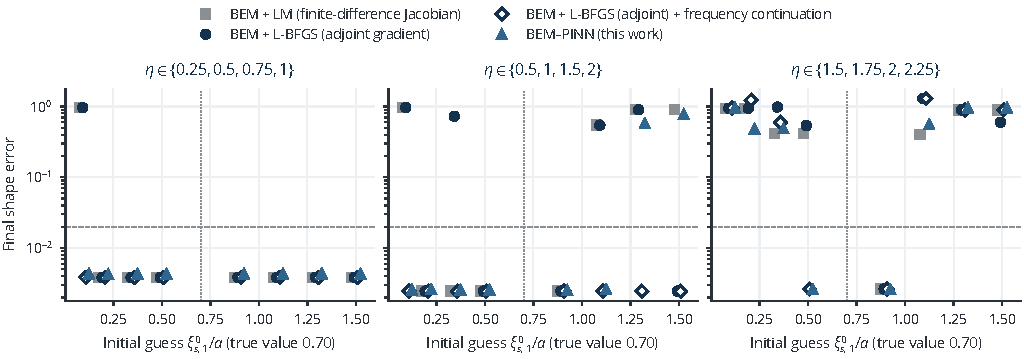
\includegraphics[width=6.5in]{figures/basin_of_attraction.pdf}
    \caption{Basin of attraction (surface reconstruction, 1\% noise): final shape error against the first sine coefficient of the initial guess, for three frequency bands. Markers are shifted horizontally for visibility. The dotted line is the true value and the dashed line the convergence threshold of 2\%.}
    \label{fig:basin}
\end{figure*}

Table~\ref{tab:basin} and Fig.~\ref{fig:basin} show the results. In the low band, every solver converges from every start, except LM-FD and L-BFGS-adj without continuation from $\xi^0_{s,1}=0.1$. In the intermediate band, the solvers without continuation converge from four starts, L-BFGS-adj with continuation from all eight, and the BEM--PINN from six: it fails from the two starts farthest above the true geometry ($\xi^0_{s,1}=1.3$ and 1.5), from which even L-BFGS-adj without continuation converges in one case. In the high band, L-BFGS-adj with continuation and the BEM--PINN both converge only from $\xi^0_{s,1}=0.5$ and 0.9, the two starts closest to the true value, and the other solvers only from 0.9. The BEM--PINN is therefore never more robust than the adjoint quasi-Newton solver with the same continuation, and it is less robust in the intermediate band. To exclude an unfavourable network initialization, we repeated four of the failed cases ($\xi^0_{s,1}=1.3$ and 1.5 in the intermediate band, 0.2 and 1.1 in the high band) with two further random seeds; all eight runs failed, with final shape errors of 48--77\%, close to those of the first seed.

The training histories show how the relaxation behaves. In every converged run the boundary residual at the end of the training is $L_{BC}=4\times10^{-6}$--$1.3\times10^{-5}$, below the data misfit ($7$--$8\times10^{-5}$). In every failed run it is $7\times10^{-3}$--$1.9\times10^{-2}$, three orders of magnitude larger and above the data misfit ($2$--$6\times10^{-3}$): the network has reduced the data misfit by moving the densities away from the solution of the BEM system for the current geometry, not by moving the geometry towards the true one, and the final state is not a physical solution. The enlarged search space thus does not lead the iterates to the global minimum; it adds directions along which the data can be fitted without the geometry, as in the three-dimensional case. In addition, the pre-training at the initial guess places the network on the constraint $\mathbf{A}\boldsymbol{\phi}=\mathbf{b}$ before the geometry is released, so at the beginning of the joint training the BEM--PINN follows approximately the same path as the reduced formulation, and the frequency continuation, not the relaxation, determines which minimum is reached.

\subsection{The hybrid method as a prototyping tool}\label{sec:prototype}

Speed and robustness are not the advantages of the hybrid method, but the experiments above point to a different one: the effort needed to set up a new inversion. In research practice, most of the work in an inverse problem goes into trying variants of the model (other data, parametrizations, unknowns or operators) before a final formulation is chosen. Each variant changes the sensitivities; an implementation based on explicit derivatives may therefore need new shape and material sensitivities or adjoint equations. Figure~\ref{fig:methodology_scheme} compares the two workflows as implemented here. In the BEM--PINN (Fig.~\ref{fig:methodology_scheme}a), the geometry, the assembly, the data misfit and the penalty are differentiable functions that enter a single loss; the dashed boxes identify modular components that can be changed when testing a variant, and the optimizer needs the action of the boundary operator, $\mathbf{A}\hat{\boldsymbol{\phi}}$, and its automatic derivative. The adjoint solver (Fig.~\ref{fig:methodology_scheme}b) shares the same differentiable geometry, assembly and misfit, but it also needs the gradient of the solution of the linear system, $\boldsymbol{\phi}=\mathbf{A}^{-1}\mathbf{b}$, that is, an adjoint solve.

As an example of a change of data type, we repeated the three inversions of Section~\ref{sec:inverse_results} with amplitude-only records, $|u^{obs}_r|$, as would be the case for spectral amplitudes from unsynchronized stations without reliable phase. The only modification of the code is the data residual, $|u(\mathbf{x}_r)|-|u^{obs}_r|$ instead of $u(\mathbf{x}_r)-u^{obs}_r$ in $L_d$ (a few lines in one function), which is shared by all solvers; noise is added to the complex records before the amplitude is taken, and all other settings are those of Section~\ref{sec:setup}. Table~\ref{tab:prototype} shows that the BEM--PINN worked without any further change or tuning: its shape errors (0.31--1.92\%) are comparable to those obtained with complex records (Table~\ref{tab:inverse}) and to those of the classical solvers with amplitude data, the boundary residual at the end of training ($L_{BC}=2.7\times10^{-6}$--$3.3\times10^{-5}$) remained below the data misfit in every case, and the material parameters of the joint problem were recovered with errors below 1.7\%. The classical solvers reached the same accuracy, except L-BFGS-adj without continuation in the joint problem, which failed at every noise level (shape error 110\%); with complex data it had failed at 0 and 1\% noise.

\begin{table}[ht!]
\centering
\caption{Inversion from amplitude-only records $|u^{obs}_r|$: shape error for three noise levels and mean wall-clock time per inversion. Same configuration as Table~\ref{tab:inverse}; only the data residual was changed.}
\label{tab:prototype}
\scriptsize
\setlength{\tabcolsep}{4pt}
\begin{tabular}{llcccc}
\toprule
 & & \multicolumn{3}{c}{shape error (\%)} & \\
\cmidrule(lr){3-5}
Problem & Solver & 0\% & 1\% & 3\% & time (s)\\
\midrule
Interface & BEM + LM (FD) & 1.30 & 1.35 & 1.53 & 0.76\\
 & BEM + L-BFGS (adjoint) & 1.30 & 1.35 & 1.53 & 0.492\\
 & BEM + L-BFGS (adjoint) + cont. & 1.30 & 1.35 & 1.53 & 0.884\\
 & BEM--PINN & 1.33 & 1.30 & 1.92 & 251\\
\midrule
Free surface & BEM + LM (FD) & 0.28 & 0.34 & 0.50 & 0.836\\
 & BEM + L-BFGS (adjoint) & 0.28 & 0.34 & 0.50 & 0.375\\
 & BEM + L-BFGS (adjoint) + cont. & 0.28 & 0.34 & 0.50 & 0.689\\
 & BEM--PINN & 0.31 & 0.36 & 0.47 & 198\\
\midrule
Joint & BEM + LM (FD) & 0.34 & 0.66 & 1.34 & 1.89\\
 & BEM + L-BFGS (adjoint) & 110.04 & 110.05 & 110.09 & 0.867\\
 & BEM + L-BFGS (adjoint) + cont. & 0.34 & 0.66 & 1.34 & 1.33\\
 & BEM--PINN & 0.55 & 0.67 & 1.48 & 191\\
\bottomrule
\end{tabular}

\end{table}

This example also shows the limit of the argument. The change of data type was equally simple for L-BFGS-adj, because its gradient is obtained by reverse-mode differentiation through the same differentiable BEM and the LU solve; most of the flexibility therefore comes from the differentiable BEM, not from the network. What is specific to the hybrid method is that it never differentiates through a linear solve. In our implementation automatic differentiation handles the dense LU solve, whereas the GMRES routine of Section~\ref{sec:iterative} required a custom backward pass using an adjoint GMRES solve with $\mathbf{A}^H$ and the corresponding matrix gradient. Other iterative or fast BEM back-ends likewise need a differentiable solve or an adjoint implementation for the reduced formulation, depending on the software used. The BEM--PINN does not require differentiating the solve, but still needs the operator product $\mathbf{A}\hat{\boldsymbol{\phi}}$ to be differentiable with respect to the network and the unknowns. In exchange, each prototype costs minutes instead of seconds (Table~\ref{tab:prototype}), and the boundary residual must be monitored to detect non-physical solutions (Section~\ref{sec:basin}). One possible workflow is therefore to explore new formulations with the hybrid method and then use an adjoint quasi-Newton solver, reusing the differentiable geometry, assembly, data misfit and regularization.

%-------------------------------------------------------------------------------
\section{Discussion}\label{sec:discussion}
\fancyhead[RO]{\textit{Discussion}\, / \thepage}
%-------------------------------------------------------------------------------

The forward reproduction confirms the main claim of \citet{wu_novel_2026}: a Fourier-feature network can represent the source densities of the indirect BEM accurately, and when trained long enough it converges to the same solution as the direct solve of the collocation system. Its errors are therefore bounded by the BEM discretization and not by the network. This holds at the excitations used for training; between training frequencies, the network did not interpolate accurately in our tests, so for multi-frequency studies each frequency of interest has to be part of the training set. We obtained smaller errors than those reported in the original work for the canyon and the hill, mainly because of the half-space Green's function and the curvature correction of the self term, which also apply to the direct IBEM. On the other hand, the comparison of computational times does not reproduce the speed-up reported by \citet{wu_novel_2026} for multi-frequency evaluations. With an efficient assembly, the direct IBEM solves the problems considered here in hundredths of a second, so training a network, which takes minutes, cannot be competitive in two dimensions for a fixed set of frequencies; the speed-up reported in the original work is probably related to their BEM implementation, whose cost (about 0.9~h per frequency) is several orders of magnitude larger than that of our implementation for problems of the same size.

For inversion, the hybrid method achieves its main methodological goals. Shape and material sensitivities are obtained by automatic differentiation without deriving shape derivatives or adjoint equations, the forward and inverse problems are solved simultaneously, the wave radiation is represented exactly through the Green's functions, and the reconstructions are as accurate as those of the classical solvers under the same data and discretization. Its limitation is computational: in two dimensions, the cost is dominated by the kernel assembly, which the BEM--PINN must repeat at every step, so not solving the linear system brings no benefit, and the stochastic optimization of the network needs many more iterations than Gauss--Newton or quasi-Newton methods on a handful of shape parameters. We also note that the differentiable implementation of the BEM used by the hybrid method provides, as a by-product, the exact adjoint gradients that make the classical L-BFGS-adj solver the fastest option in our tests.

Can the hybrid method be advantageous? We looked for such a regime in three settings: the small two-dimensional problems solved with LU factorizations, the same problems solved with iterative solvers as for models whose matrix cannot be factorized (Section~\ref{sec:iterative}), and a three-dimensional model (Section~\ref{sec:three_d}). In none of them was the hybrid method cheaper than the adjoint-based classical solver, and the reason is the same in all cases. The cost of every method is dominated by the evaluation of the boundary integral operator (assembly or matrix-vector products), not by the linear solve; the BEM--PINN avoids the solve but needs one operator evaluation per loss evaluation and several thousand loss evaluations, whereas an adjoint quasi-Newton method needs a few tens of objective evaluations and, with a preconditioned iterative solver, ten to a hundred operator products per solve. Because the number of products of the hybrid method does not depend on the mesh size, while that of the iterative classical solvers grows slowly, a crossover exists in principle, but our measurements place it at about $10^6$ unknowns in two dimensions, beyond the accuracy that a fixed training budget can deliver. A favourable situation would require forward problems that are much harder for preconditioned iterative solvers than for gradient-based training; this is unlikely, because minimizing $\|\mathbf{A}\boldsymbol{\phi}-\mathbf{b}\|^2$ squares the condition number of $\mathbf{A}$, and indeed the network failed where the system was nearly singular. The hybrid method does reduce the cost relative to finite-difference inversion when the number of unknowns $P$ is large, since its cost does not depend on $P$, but a differentiable BEM with adjoint gradients achieves the same independence at a much lower cost. Nor did we find an advantage in robustness (Section~\ref{sec:basin}): penalizing the boundary conditions instead of enforcing them did not enlarge the basin of attraction relative to the adjoint quasi-Newton solver with the same frequency continuation, because the additional freedom was used to fit the data with non-physical densities. Relaxed formulations that do mitigate local minima, such as wavefield reconstruction inversion \citep{vanLeeuwen2013}, eliminate the field variables by solving a least-squares problem for every geometry and control the weight of the physics penalty explicitly; in the BEM--PINN the densities are adjusted by stochastic gradient steps together with the geometry, with a fixed weight, so the same benefit cannot be expected without changing the formulation. In our view, the practical value of the hybrid approach is therefore not computational speed or robustness but simplicity: the same differentiable boundary integral model provides forward solutions, sensitivities and inversion without adjoint derivations or linear solvers, which makes it a convenient prototyping tool (Section~\ref{sec:prototype}), particularly for matrix-free or fast BEM operators whose linear solve cannot be differentiated automatically.

Several aspects of the formulation require care regardless of the solver. First, the single-layer representation with the half-space Green's function can be singular at the interior Dirichlet eigenvalues of the closed contour formed by the free surface and its image. For the V-shaped canyon this happens at $\eta=1$, $1.58$ and $2$, including the benchmark frequency of \citet{wu_novel_2026}: there, both the IBEM and the network converge to a wrong solution (errors of order one against the formulation with a meshed flat surface), and a reference computed with the same formulation does not reveal the problem. We therefore used the formulation of \citet{wu_novel_2026}, with a meshed flat surface and the full-space Green's function, for the V-shaped canyon. The inversion systems used here are well conditioned in the frequency band considered, but a combined-layer formulation would remove this risk \citep{Colton2013}. Second, the densities of the network are not exact solutions of the discrete system, and this residual interacts with the data misfit; monitoring $L_{BC}$ during the joint training is necessary to ensure that the geometry is not fitted to a non-physical density. Third, the robustness of the joint identification depends on the optimization strategy (frequency continuation, bounds) at least as much as on the solver.

This study has limitations. The comparison with \citet{Bignardi2012}, \citet{Wang2018} and \citet{Bonnet2009} is indirect: those works address in-plane or three-dimensional elastodynamics, and we implemented their inversion algorithms for the antiplane problem rather than reproducing their numerical results; \citet{Wang2018} uses a linearized Born inversion of Rayleigh-wave reflection coefficients that has no direct counterpart in our setting and is not included. All computations ran on a laptop CPU; the training times of the networks would be shorter on a GPU, but the cost ratio per iteration with respect to the adjoint solver would not change because both are dominated by the same assembly. Each case of Sections~\ref{sec:inverse_results}--\ref{sec:three_d} was run with one network initialization and one noise realization; in the basin-of-attraction test, three seeds gave the same outcome in the four cases repeated. The robustness study considered only surface reconstruction with one-parameter families of initial guesses, so it does not exclude that the relaxation helps in other problems or for other perturbations of the initial geometry. Finally, the two-dimensional examples use a smooth hill with four sine coefficients per curve, and the three-dimensional study uses a scalar (acoustic-type) model of a canyon with six coefficients; three-dimensional elastodynamics, more complex geometries and real records remain to be studied.

%-------------------------------------------------------------------------------
\section{Conclusions}\label{sec:conclusions}
\fancyhead[RO]{\textit{Conclusions}\, / \thepage}
%-------------------------------------------------------------------------------

We applied a hybrid BEM--PINN method, in which a Fourier-feature network represents the source densities of an indirect BEM, to three inverse SH-wave problems in irregular topographies: interface identification, free-surface reconstruction, and joint identification of geometry and material properties. The geometric and material unknowns are trained jointly with the network, and their gradients are obtained by automatic differentiation through a differentiable BEM assembly with the half-space Green's function.

The forward benchmarks of \citet{wu_novel_2026} were reproduced with errors between $3.6\times10^{-4}$ and $4.7\times10^{-3}$, and the network converged to the direct BEM solution in all cases. In the inverse problems, the hybrid method reached the same accuracy as two classical BEM inversion strategies (Levenberg--Marquardt with finite differences and L-BFGS with adjoint gradients) using the same data and discretization: shape errors of 1--2\% for the buried interface, 0.35--0.6\% for the free surface, and below 0.7\% for geometry and material properties together, with up to 3\% noise. Its robustness in the joint problem was due to frequency continuation, which also makes the classical quasi-Newton solver robust.

The hybrid method was two to three orders of magnitude slower than the classical solvers for these two-dimensional problems. The cost analysis shows that one joint training step costs as much as one adjoint gradient, because both are dominated by the assembly of the boundary integral kernels, so avoiding the linear solve does not pay off unless the dense solve dominates, which in our measurements happens only above a few thousand unknowns. The method is therefore attractive for its simplicity, since no sensitivity or adjoint derivations are required, rather than for its speed. We searched for a regime in which the hybrid method pays off. With preconditioned GMRES for the classical solvers, the number of operator products of the hybrid method is independent of the mesh size but remains 6 to 10 times larger than that of L-BFGS with adjoint gradients up to 960 unknowns, and the fitted trends would only cross at about $10^6$ unknowns. In a three-dimensional scalar model of a canyon, validated against the exact solution for a hemispherical canyon, the hybrid method needed 25 times more products and reached depth errors of 5.5--7.2\%, against 0.9--4.6\% for the classical solvers, because the network did not solve the forward problem accurately enough relative to the weak signature of the canyon in the data. Our initial hypothesis, that avoiding the linear solve would make the inversion cheaper, is therefore rejected for the problems studied. We also tested whether the relaxed formulation of the hybrid method, in which the boundary conditions are only penalized, enlarges the basin of attraction. Over eight initial guesses and three frequency bands of surface reconstruction, the hybrid method converged from 8, 6 and 2 starts, against 8, 8 and 2 for L-BFGS with adjoint gradients and the same frequency continuation, and the failed runs ended with boundary residuals larger than the data misfit. The advantage of the hybrid approach is thus neither speed nor robustness but a single differentiable model that provides forward solutions, sensitivities and inversion without adjoint derivations or linear solvers. This makes it useful for prototyping: switching to amplitude-only records required changing only the data residual, and the hybrid method recovered geometry and material properties with errors below 2\% without further tuning. Because it needs only the action of the boundary operator, it also works with operators whose linear solve has no automatic adjoint, such as iterative or fast BEM solvers. We therefore suggest using it to explore new formulations and switching to an adjoint quasi-Newton solver on the same differentiable BEM for production inversions. Future work should address three-dimensional elastodynamics, GPU implementations, combined-layer formulations that avoid irregular frequencies, training strategies that keep the boundary residual below the data misfit, and field data.

\section*{Code availability}
The implementation (differentiable indirect BEM, analytical solutions, BEM--PINN and classical solvers) and the scripts that generate all figures and tables are in the \texttt{code/} directory of the project repository.

%-------------------------------------------------------------------------------
% References
%-------------------------------------------------------------------------------
\bibliography{refs}

\end{document}
